%%% Lecture 1 Slides %%%

\documentclass{beamer}

%\documentclass[handout]{beamer}
%\usepackage{pgfpages}
%\pgfpagesuselayout{2 on 1}[a4paper,border shrink=5mm]
%\pgfpagesuselayout{1 on 1}[a4paper,border shrink=5mm]



\usepackage{amssymb}
\usepackage{amsmath}
\usepackage{mathtools}
\usepackage{tikz}
\usetikzlibrary{shapes,arrows}
\usetikzlibrary{positioning}
\usetikzlibrary{trees}
\usepackage{pgfplots}
\usepackage{pdflscape}
\usepackage{graphicx}
\usepackage{colortbl}
\usepackage{listings}
\usepackage{adjustbox}

\DeclarePairedDelimiter{\ceil}{\lceil}{\rceil}

\newcommand{\bs}{\boldsymbol}
\newcommand{\mb}{\mathbf}
\newcommand{\indep}{{\bot\negthickspace\negthickspace\bot}}
\newcommand{\notindep}{{\bot\negthickspace\negthickspace\bot}{\negthinspace
  \negmedspace \negthickspace \negthickspace \diagup
  \;}}
\renewcommand{\S}{\mb{S}}
\usepackage{color}
\definecolor{direct}{HTML}{FF0000}
\definecolor{indirect}{HTML}{FF9999}
\definecolor{dirin}{HTML}{990000}
\definecolor{control}{HTML}{999999}
\definecolor{directE}{HTML}{ED1C24}
\definecolor{indirectE}{HTML}{F69679}
\definecolor{controlE}{HTML}{999999}

%\defV{{\rm Var}\,}
\def\E{{\rm E}\,}
\def\arg{{\rm arg}\,}
\def\Cov{{\rm Cov}\,}
\def\N{{\rm N}\,}
\newcommand{\plim}{{\rm plim} \,}
\DeclareMathOperator*{\argmin}{arg\,min}
\newcommand{\X}{\mathbf{X}}
\newcommand{\Y}{\mathbf{Y}}
\newcommand{\Z}{\mathbf{Z}}
\newcommand{\I}{\mathbf{I}}
\newcommand{\V}{\mathbf{\Omega}}
\newcommand{\W}{\mathbf{W}}
\newcommand{\R}{\mathbf{R}}
\newcommand{\A}{\mathbf{A}}
\newcommand{\B}{\mathbf{B}}
\newcommand{\D}{\mathbf{D}}
\newcommand{\T}{\mathbf{T}}
\newcommand{\F}{\mathbf{F}}
\renewcommand{\O}{\mathbf{O}}
\renewcommand{\H}{\mathbf{H}}
\newcommand{\g}{\mathbf{g}}
\renewcommand{\r}{\mathbf{r}}
\newcommand{\s}{\mathbf{s}}
\newcommand{\uu}{\mathbf{u}}
\newcommand{\w}{\mathbf{w}}
\newcommand{\x}{\mathbf{x}}
\newcommand{\vv}{\mathbf{v}}
\newcommand{\z}{\mathbf{z}}
\newcommand{\y}{\mathbf{y}}

\newcommand{\bi}{\begin{itemize}}
\newcommand{\ei}{\end{itemize}}
\newcommand{\be}{\begin{enumerate}}
\newcommand{\ee}{\end{enumerate}}

\newcommand{\Beta}{\boldsymbol{\beta}}
\newcommand{\btheta}{\boldsymbol{\theta}}
\newcommand{\bgamma}{\boldsymbol{\gamma}}
\newcommand{\bpi}{\boldsymbol{\pi}}
\newcommand{\arrowp}{\stackrel{p}{\rightarrow}}
\newcommand{\arrowd}{\stackrel{d}{\rightarrow}}
\newcommand{\0}{\mathbf{0}}
\newcommand{\bP}{\mathbf{P}}
\newcommand{\nn}{\nonumber}
\def\S{{\sigma}}
\def\Supp{{\rm Supp}\,}


\newcommand\independent{\protect\mathpalette{\protect\independenT}{\perp}}
\def\independenT#1#2{\mathrel{\rlap{$#1#2$}\mkern2mu{#1#2}}}

\newcommand{\vsf}{\vspace{.5cm}}

\usepackage[english]{babel}
% or whatever

\usepackage[latin1]{inputenc}
% or whatever

\usepackage{times}
\usepackage[T1]{fontenc}
\setbeamertemplate{footline}[page number]{}
\setbeamertemplate{navigation symbols}{}


\title[Lecture 4: Inference for Subpopulation Proportions and Differences] % (optional, use only with long paper titles)
{Lecture 4: Inference for Subpopulation Proportions and Differences}


\begin{document}

\begin{frame}
  \titlepage
\end{frame}


\frame{
\frametitle{Review}

\begin{itemize}
\item In previous lectures, we discussed learning about population proportions and means based on a random sample (with replacement) from the population. \pause
\item We saw that for large enough sample sizes, our sample proportion/mean was likely to be close to the population proportion/mean. \pause
\item We also demonstrated that we could predict how close we might by using confidence intervals. \pause
\item We explored a bootstrapping approach and a plug-in approach to producing confidence intervals.  
\end{itemize}

}

\frame{
\frametitle{In this lecture}

\begin{itemize}
\item In this lecture, we discuss learning subpopulation proportions and differences between subpopulation proportions based on a random sample (with replacement) from the population. \pause
\item Returning to the turnout example, we will consider Black turnout and the difference between Black and non-Black turnout in the 2020 Georgia presidential election. \pause
\item Even when the overall sample size is fixed (625 for our example), different random samples will produce different subgroup sample sizes, and this adds a layer of complexity.  \pause
\item This complexity will not complicate our analysis much but it does complicate the justification for the analysis.
\end{itemize}

}





\frame{
\frametitle{2020 Presidential Election Turnout in Georgia}

We return to the turnout application, but we are now interested in Black turnout and Black turnout in comparison to non-Black turnout. Recall that ... 
\begin{itemize}
\item based on a survey of 625 registered voters a week before the election, we got a turnout rate of .68, 
\item after the election, we found that the turnout rate among all registered voters was .70
\end{itemize} \pause
Suppose we also want to predict Black turnout and the difference between Black and non-Black turnout. \pause
\begin{itemize}
\item in our survey of 625 registered voters, 184 were Black with a turnout rate of .71 and 441 were non-Black with a turnout rate of .67.   \pause
\item after the election, we found that the turnout rate among the 30\% of registered voters who were black was .74 and among the 70\% of non-Black registered voters was .68.
\end{itemize}


}

\frame{
\frametitle{Four Questions}

\begin{enumerate}
\item .71 is close to the Black turnout rate of .74. Did we get lucky?  \pause
\item Could we have predicted how close we would get to .74 before the election? \pause 
\item The survey turnout gap of .04 is close to the population turnout gap of .06. Did we get lucky? \pause
\item Could we have predicted how close we would get to a .06 turnout gap before the election? 
\end{enumerate} 

}

\frame{
\frametitle{Sampling Distribution for Black Turnout Proportion}
\footnotesize

Let the variable $X$ take the value 1 if Black and 0 if non-Black
\begin{center}
\begin{tabular}{r|r|r|r|r|r|r}
$i$ & \multicolumn{1}{r|}{1} & \multicolumn{1}{r|}{2}   & $\dots$ & \multicolumn{1}{r|}{625} &  &  \\
\visible<2->{$s$} & $Y_1,X_1$  & $Y_2,X_2$   & $\dots$  & $Y_{625},X_{625}$  & $\overline{Y}_{625}$ &  $\frac{\sum_{i=1}^{625}Y_{i}X_{i}}{\sum_{i=1}^{625}X_{i}} $\\
\hline
\visible<2->{1}  & 1,0 & 1,1   & $\dots$  & 0,0 & .68 & .69\\
\visible<2->{2} & \visible<2->{0,0} & \visible<2->{1,0}   & \visible<2->{$\dots$}  & \visible<2->{1,1} & \visible<2->{.70} & \visible<2->{.72} \\
\visible<3->{3} & \visible<3->{1,0}& \visible<3->{1,1}  & \visible<3->{$\dots$} & \visible<3->{0,1} & \visible<3->{.75} & \visible<3->{.76} \\
\visible<3->{4} &  \visible<3->{1,1}& \visible<3->{1,0} & \visible<3->{$\dots$}  & \visible<3->{0,0} & \visible<3->{.73} & \visible<3->{.73} \\
\visible<3->{5}  & \visible<3->{0,0} & \visible<3->{0,0}  & \visible<3->{$\dots$}  & \visible<3->{1,1} & \visible<3->{.69} & \visible<3->{.71} \\
\visible<3->{$\vdots$}  & \visible<3->{$\vdots$} & \visible<3->{$\vdots$}   & \visible<3->{$\vdots$} & \visible<3->{$\vdots$} &  \visible<3->{$\vdots$}&  \visible<3->{$\vdots$} \\ 
\visible<3->{1 mil} & \visible<3->{1,0} & \visible<3->{0,1}& \visible<3->{$\dots$}  & \visible<3->{1,1} & \visible<3->{.74} & \visible<3->{.75} \\
 \visible<3->{$\vdots$}   & \visible<3->{$\vdots$} & \visible<3->{$\vdots$}  & \visible<3->{$\vdots$} & \visible<3->{$\vdots$}  & \visible<3->{$\vdots$} & \visible<3->{$\vdots$} \\ 
\hline
\visible<1->{$f_{\cdot}(\cdot)$} & \multicolumn{1}{r|}{\visible<1->{}} & \multicolumn{1}{r|}{\visible<1->{}}  &$\dots$ & \multicolumn{1}{r|}{\visible<1->{}} & \visible<1->{$N(.7,\frac{.7 \cdot (1-.7)}{n})$} \\
\visible<1->{$E_{\cdot}(\cdot)$} & \multicolumn{1}{r|}{\visible<1->{}} & \multicolumn{1}{r|}{\visible<1->{}}  &$\dots$ & \multicolumn{1}{r|}{\visible<1->{}} & \visible<1->{$.7$} \\
\visible<1->{$V_{\cdot}(\cdot)$} & \multicolumn{1}{r|}{\visible<1->{}} & \multicolumn{1}{r|}{\visible<1->{}}  &$\dots$ & \multicolumn{1}{r|}{\visible<1->{}} & \visible<1->{$.7 \cdot (1-.7)$} \\
\end{tabular}
\end{center}

Note that $\sum_{i=1}^{625}Y_{i}X_{i}$ is not a binomial RV, so we use the general CLT approach.
}

\frame{
\frametitle{What can we learn?}
\begin{table}[h]
\begin{center}
{\scriptsize
\begin{tabular}{r|r|r|r|r|r} %cc
$i$ & \multicolumn{1}{r|}{1} & \multicolumn{1}{r|}{2}   & $\dots$ & \multicolumn{1}{r|}{2258} & \\ % & \multicolumn{1}{c}{$MoE$}& \multicolumn{1}{c}{95\% CI}  \\
$s$  & $Y_1$  & $Y_2$   & $\dots$  & $Y_{2258}$  & $\overline{Y}_{2258}$ \\ % & $2\cdot\sqrt{\frac{\overline{Y}_{625}(1-\overline{Y}_{625})}{625}}$ & $\overline{Y}_{625} \pm MoE$ \\
\hline
1 & 37,006 & 108,811   & $\dots$  &  49,001  & 135,406   \\ %& \visible<2->{.037} & \visible<3->{[.643,.717]}\\
\visible<1->{2} & \visible<1->{?} & \visible<1->{?}   & \visible<1->{$\dots$}  & \visible<1->{?} & \visible<1->{?} \\ %& \visible<2->{.037}  & \visible<3->{[.663,.737]}\\
\visible<1->{3} & \visible<1->{?} & \visible<1->{?}  & \visible<1->{$\dots$}  & \visible<1->{?} & \visible<1->{?} \\ %& \visible<2->{.035} & \visible<3->{[.715,.785]}\\
\visible<1->{4} & \visible<1->{$\vdots$} & \visible<1->{$\vdots$} & \visible<1->{$\dots$}  & \visible<1->{$\vdots$} & \visible<1->{$\vdots$} \\ %& \visible<2->{.036} & \visible<3->{[.694,.766]}\\
\visible<1->{5} & \visible<1->{$\vdots$} & \visible<1->{$\vdots$}  & \visible<1->{$\dots$}  & \visible<1->{$\vdots$} & \visible<1->{$\vdots$} \\ %& \visible<2->{.037} & \visible<3->{[.653,.727]}\\
\visible<1->{$\vdots$} & \visible<1->{$\vdots$}  & \visible<1->{$\vdots$} & \visible<1->{$\vdots$} & \visible<1->{$\vdots$}  & \visible<1->{$\vdots$} \\ % & \visible<2->{$\vdots$} & \visible<3->{$\vdots$}  \\
\visible<1->{1 mil}  & \visible<1->{?} & \visible<1->{?} & \visible<1->{$\dots$}  & \visible<1->{?} & \visible<1->{?} \\ %& \visible<2->{.035}& \visible<3->{[.705,.775]}\\
 \visible<1->{$\vdots$}  & \visible<1->{$\vdots$}  & \visible<1->{$\vdots$} & \visible<1->{$\vdots$} & \visible<1->{$\vdots$}  & \visible<1->{$\vdots$} \\ % & \visible<2->{$\vdots$} & \visible<3->{$\vdots$}\\
\hline
\visible<1->{$f_{\cdot}(\cdot)$} & \multicolumn{1}{r|}{\visible<1->{?}} & \multicolumn{1}{r|}{\visible<1->{?}}  &$\dots$ & \multicolumn{1}{r|}{\visible<1->{?}} & \visible<1->{\textcolor{red}{?}} \\
\visible<1->{$E_{\cdot}(\cdot)$} & \multicolumn{1}{r|}{\visible<1->{$\mu$}} & \multicolumn{1}{r|}{\visible<1->{$\mu$}}  &$\dots$ & \multicolumn{1}{r|}{\visible<1->{$\mu$}} & \visible<1->{\textcolor{red}{?}} \\
\visible<1->{$V_{\cdot}(\cdot)$} & \multicolumn{1}{r|}{\visible<1->{$\sigma^2$}} & \multicolumn{1}{r|}{\visible<1->{$\sigma^2$}}  &$\dots$ & \multicolumn{1}{r|}{\visible<1->{$\sigma^2$}} & \visible<1->{\textcolor{red}{?}} \\
\end{tabular}}
%\caption{\emph{Sampling Distributions for $\overline{Y}_{625}$, the Margin-of-Error, and the 95\% Confidence Interval}}\label{t:samdistCI}
\end{center}
\end{table}

\begin{itemize}
\item Although we can't observe the population or the sampling distribution, we can mathematically derive certain facts about the sampling distribution. 
\item We will focus on the three red question marks.
\end{itemize}
}

\frame{
\frametitle{The Type of Distribution}
\begin{table}[h]
\begin{center}
{\scriptsize
\begin{tabular}{r|r|r|r|r|r} %cc
$i$ & \multicolumn{1}{r|}{1} & \multicolumn{1}{r|}{2}   & $\dots$ & \multicolumn{1}{r|}{2258} & \\ % & \multicolumn{1}{c}{$MoE$}& \multicolumn{1}{c}{95\% CI}  \\
$s$  & $Y_1$  & $Y_2$   & $\dots$  & $Y_{2258}$  & $\overline{Y}_{2258}$ \\ % & $2\cdot\sqrt{\frac{\overline{Y}_{625}(1-\overline{Y}_{625})}{625}}$ & $\overline{Y}_{625} \pm MoE$ \\
\hline
1 & 37,006 & 108,811   & $\dots$  &  49,001  & 135,406   \\ %& \visible<2->{.037} & \visible<3->{[.643,.717]}\\
\visible<1->{2} & \visible<1->{?} & \visible<1->{?}   & \visible<1->{$\dots$}  & \visible<1->{?} & \visible<1->{?} \\ %& \visible<2->{.037}  & \visible<3->{[.663,.737]}\\
\visible<1->{3} & \visible<1->{?} & \visible<1->{?}  & \visible<1->{$\dots$}  & \visible<1->{?} & \visible<1->{?} \\ %& \visible<2->{.035} & \visible<3->{[.715,.785]}\\
\visible<1->{4} & \visible<1->{$\vdots$} & \visible<1->{$\vdots$} & \visible<1->{$\dots$}  & \visible<1->{$\vdots$} & \visible<1->{$\vdots$} \\ %& \visible<2->{.036} & \visible<3->{[.694,.766]}\\
\visible<1->{5} & \visible<1->{$\vdots$} & \visible<1->{$\vdots$}  & \visible<1->{$\dots$}  & \visible<1->{$\vdots$} & \visible<1->{$\vdots$} \\ %& \visible<2->{.037} & \visible<3->{[.653,.727]}\\
\visible<1->{$\vdots$} & \visible<1->{$\vdots$}  & \visible<1->{$\vdots$} & \visible<1->{$\vdots$} & \visible<1->{$\vdots$}  & \visible<1->{$\vdots$} \\ % & \visible<2->{$\vdots$} & \visible<3->{$\vdots$}  \\
\visible<1->{1 mil}  & \visible<1->{?} & \visible<1->{?} & \visible<1->{$\dots$}  & \visible<1->{?} & \visible<1->{?} \\ %& \visible<2->{.035}& \visible<3->{[.705,.775]}\\
 \visible<1->{$\vdots$}  & \visible<1->{$\vdots$}  & \visible<1->{$\vdots$} & \visible<1->{$\vdots$} & \visible<1->{$\vdots$}  & \visible<1->{$\vdots$} \\ % & \visible<2->{$\vdots$} & \visible<3->{$\vdots$}\\
\hline
\visible<1->{$f_{\cdot}(\cdot)$} & \multicolumn{1}{r|}{\visible<1->{?}} & \multicolumn{1}{r|}{\visible<1->{?}}  &$\dots$ & \multicolumn{1}{r|}{\visible<1->{?}} & \visible<1->{\textcolor{red}{N(?,?)}} \\
\visible<1->{$E_{\cdot}(\cdot)$} & \multicolumn{1}{r|}{\visible<1->{$\mu$}} & \multicolumn{1}{r|}{\visible<1->{$\mu$}}  &$\dots$ & \multicolumn{1}{r|}{\visible<1->{$\mu$}} & \visible<1->{\textcolor{red}{?}} \\
\visible<1->{$V_{\cdot}(\cdot)$} & \multicolumn{1}{r|}{\visible<1->{$\sigma^2$}} & \multicolumn{1}{r|}{\visible<1->{$\sigma^2$}}  &$\dots$ & \multicolumn{1}{r|}{\visible<1->{$\sigma^2$}} & \visible<1->{\textcolor{red}{?}} \\
\end{tabular}}
%\caption{\emph{Sampling Distributions for $\overline{Y}_{625}$, the Margin-of-Error, and the 95\% Confidence Interval}}\label{t:samdistCI}
\end{center}
\end{table}

Property \#1: {\it The sampling distribution of the sample mean is approximately normal when $n$ is large.}
\begin{itemize}
\item The approximate normality result comes from the central limit theorem (CLT). 
\item We know that $\overline{Y}_{2258} \sim^{approx} N(?,?)$, but still don't know the mean or the variance of this distribution. 
\end{itemize}
}



%\frame{
%\frametitle{Sampling Distribution for the Sample Mean}
%\begin{table}[h]
%\begin{center}
%{\scriptsize
%\begin{tabular}{r|r|r|r|r|r} %cc
%$i$ & \multicolumn{1}{r|}{1} & \multicolumn{1}{r|}{2}   & $\dots$ & \multicolumn{1}{r|}{2258} & \\ % & \multicolumn{1}{c}{$MoE$}& \multicolumn{1}{c}{95\% CI}  \\
%$s$  & $Y_1$  & $Y_2$   & $\dots$  & $Y_{2258}$  & $\overline{Y}_{2258}$ \\ % & $2\cdot\sqrt{\frac{\overline{Y}_{625}(1-\overline{Y}_{625})}{625}}$ & $\overline{Y}_{625} \pm MoE$ \\
%\hline
%1 & 37,006 & 108,811   & $\dots$  &  49,001  & 135,406   \\ %& \visible<2->{.037} & \visible<3->{[.643,.717]}\\
%\visible<2->{2} & \visible<2->{152,001} & \visible<2->{174,261}   & \visible<2->{$\dots$}  & \visible<2->{75,105} & \visible<2->{135,956} \\ %& \visible<2->{.037}  & \visible<3->{[.663,.737]}\\
%\visible<2->{3} & \visible<2->{4,800} & \visible<2->{52,000}  & \visible<2->{$\dots$}  & \visible<2->{169,900} & \visible<2->{133,790} \\ %& \visible<2->{.035} & \visible<3->{[.715,.785]}\\
%\visible<2->{4} & \visible<2->{$\vdots$} & \visible<2->{$\vdots$} & \visible<2->{$\dots$}  & \visible<2->{$\vdots$} & \visible<2->{$\vdots$} \\ %& \visible<2->{.036} & \visible<3->{[.694,.766]}\\
%\visible<2->{5} & \visible<2->{$\vdots$} & \visible<2->{$\vdots$}  & \visible<2->{$\dots$}  & \visible<2->{$\vdots$} & \visible<2->{$\vdots$} \\ %& \visible<2->{.037} & \visible<3->{[.653,.727]}\\
%\visible<2->{$\vdots$} & \visible<2->{$\vdots$}  & \visible<2->{$\vdots$} & \visible<2->{$\vdots$} & \visible<2->{$\vdots$}  & \visible<2->{$\vdots$} \\ % & \visible<2->{$\vdots$} & \visible<3->{$\vdots$}  \\
%\visible<2->{1 mil}  & \visible<2->{80,149} & \visible<2->{36,001} & \visible<2->{$\dots$}  & \visible<2->{187,078} & \visible<2->{134,127} \\ %& \visible<2->{.035}& \visible<3->{[.705,.775]}\\
% \visible<2->{$\vdots$}  & \visible<2->{$\vdots$}  & \visible<2->{$\vdots$} & \visible<2->{$\vdots$} & \visible<2->{$\vdots$}  & \visible<2->{$\vdots$} \\ % & \visible<2->{$\vdots$} & \visible<3->{$\vdots$}\\
%\hline
%\visible<1->{$f_{\cdot}(\cdot)$} & \multicolumn{1}{r|}{\visible<1->{?}} & \multicolumn{1}{r|}{\visible<1->{?}}  &$\dots$ & \multicolumn{1}{r|}{\visible<1->{?}} & \visible<1->{?} \\
%\visible<1->{$E_{\cdot}(\cdot)$} & \multicolumn{1}{r|}{\visible<1->{$\mu$}} & \multicolumn{1}{r|}{\visible<1->{$\mu$}}  &$\dots$ & \multicolumn{1}{r|}{\visible<1->{$\mu$}} & \visible<1->{?} \\
%\visible<1->{$V_{\cdot}(\cdot)$} & \multicolumn{1}{r|}{\visible<1->{$\sigma^2$}} & \multicolumn{1}{r|}{\visible<1->{$\sigma^2$}}  &$\dots$ & \multicolumn{1}{r|}{\visible<1->{$\sigma^2$}} & \visible<1->{?} \\
%\end{tabular}}
%%\caption{\emph{Sampling Distributions for $\overline{Y}_{625}$, the Margin-of-Error, and the 95\% Confidence Interval}}\label{t:samdistCI}
%\end{center}
%\end{table}
%
%\begin{itemize}
%\item Recall that we can think of $Y_1,...,Y_n$ as $i.i.d.$ RVs.
%\item Although we don't know the distribution $f_Y(y)$ of these RVs, their expected value $E[Y]$ is the population mean $\mu$ and their variance $V[Y]$ is the population variance $\sigma^2$.
%\end{itemize}
%
%
%}


\frame{
\frametitle{What is the $E[\overline{Y}_{n}]$?}
\begin{table}[h]
\begin{center}
{\scriptsize
\begin{tabular}{r|r|r|r|r|r} %cc
$i$ & \multicolumn{1}{r|}{1} & \multicolumn{1}{r|}{2}   & $\dots$ & \multicolumn{1}{r|}{2258} & \\ % & \multicolumn{1}{c}{$MoE$}& \multicolumn{1}{c}{95\% CI}  \\
$s$  & $Y_1$  & $Y_2$   & $\dots$  & $Y_{2258}$  & $\overline{Y}_{2258}$ \\ % & $2\cdot\sqrt{\frac{\overline{Y}_{625}(1-\overline{Y}_{625})}{625}}$ & $\overline{Y}_{625} \pm MoE$ \\
\hline
1 & 37,006 & 108,811   & $\dots$  &  49,001  & 135,406   \\ %& \visible<2->{.037} & \visible<3->{[.643,.717]}\\
\visible<1->{2} & \visible<1->{?} & \visible<1->{?}   & \visible<1->{$\dots$}  & \visible<1->{?} & \visible<1->{?} \\ %& \visible<2->{.037}  & \visible<3->{[.663,.737]}\\
\visible<1->{3} & \visible<1->{?} & \visible<1->{?}  & \visible<1->{$\dots$}  & \visible<1->{?} & \visible<1->{?} \\ %& \visible<2->{.035} & \visible<3->{[.715,.785]}\\
\visible<1->{4} & \visible<1->{$\vdots$} & \visible<1->{$\vdots$} & \visible<1->{$\dots$}  & \visible<1->{$\vdots$} & \visible<1->{$\vdots$} \\ %& \visible<2->{.036} & \visible<3->{[.694,.766]}\\
\visible<1->{5} & \visible<1->{$\vdots$} & \visible<1->{$\vdots$}  & \visible<1->{$\dots$}  & \visible<1->{$\vdots$} & \visible<1->{$\vdots$} \\ %& \visible<2->{.037} & \visible<3->{[.653,.727]}\\
\visible<1->{$\vdots$} & \visible<1->{$\vdots$}  & \visible<1->{$\vdots$} & \visible<1->{$\vdots$} & \visible<1->{$\vdots$}  & \visible<1->{$\vdots$} \\ % & \visible<2->{$\vdots$} & \visible<3->{$\vdots$}  \\
\visible<1->{1 mil}  & \visible<1->{?} & \visible<1->{?} & \visible<1->{$\dots$}  & \visible<1->{?} & \visible<1->{?} \\ %& \visible<2->{.035}& \visible<3->{[.705,.775]}\\
 \visible<1->{$\vdots$}  & \visible<1->{$\vdots$}  & \visible<1->{$\vdots$} & \visible<1->{$\vdots$} & \visible<1->{$\vdots$}  & \visible<1->{$\vdots$} \\ % & \visible<2->{$\vdots$} & \visible<3->{$\vdots$}\\
\hline
\visible<1->{$f_{\cdot}(\cdot)$} & \multicolumn{1}{r|}{\visible<1->{?}} & \multicolumn{1}{r|}{\visible<1->{?}}  &$\dots$ & \multicolumn{1}{r|}{\visible<1->{?}} & \visible<1->{$N(\textcolor{red}{?},?)$} \\
\visible<1->{$E_{\cdot}(\cdot)$} & \multicolumn{1}{r|}{\visible<1->{$\mu$}} & \multicolumn{1}{r|}{\visible<1->{$\mu$}}  &$\dots$ & \multicolumn{1}{r|}{\visible<1->{$\mu$}} & \visible<1-1>{?}\hspace{-.17cm}\visible<2->{\textcolor{red}{?}} \\
\visible<1->{$V_{\cdot}(\cdot)$} & \multicolumn{1}{r|}{\visible<1->{$\sigma^2$}} & \multicolumn{1}{r|}{\visible<1->{$\sigma^2$}}  &$\dots$ & \multicolumn{1}{r|}{\visible<1->{$\sigma^2$}} & \visible<1->{?} \\
\end{tabular}}
%\caption{\emph{Sampling Distributions for $\overline{Y}_{625}$, the Margin-of-Error, and the 95\% Confidence Interval}}\label{t:samdistCI}
\end{center}
\end{table}

}


\frame{
Property \#1: {\it The sample mean is unbiased for the population mean.} The expected value of the sample mean,
$\E[\overline Y] = \mu$.

\vspace{0.2in}

Proof:
\begin{align*}
\E[\overline Y] &= \E \left[ \frac{1}{n} \left( Y_1 + ... + Y_n \right) \right] \\
& =  \\%\frac{1}{n} \E \left[ Y_1 + ... + Y_n  \right] \\
& =  \\%\frac{1}{n} \left( \E [ Y_1] + ... + \E [Y_n]  \right) \\
& =  \\%\frac{1}{n} \left( \E [ Y] + ... + \E [Y]  \right) \\
& =  \\%\frac{1}{n} n \E [ Y] \\
& = \mu.
\end{align*}

}

\frame{
\frametitle{Sample mean is unbiased for the population mean}
\begin{table}[h]
\begin{center}
{\scriptsize
\begin{tabular}{r|r|r|r|r|r} %cc
$i$ & \multicolumn{1}{r|}{1} & \multicolumn{1}{r|}{2}   & $\dots$ & \multicolumn{1}{r|}{2258} & \\ % & \multicolumn{1}{c}{$MoE$}& \multicolumn{1}{c}{95\% CI}  \\
$s$  & $Y_1$  & $Y_2$   & $\dots$  & $Y_{2258}$  & $\overline{Y}_{2258}$ \\ % & $2\cdot\sqrt{\frac{\overline{Y}_{625}(1-\overline{Y}_{625})}{625}}$ & $\overline{Y}_{625} \pm MoE$ \\
\hline
1 & 37,006 & 108,811   & $\dots$  &  49,001  & 135,406   \\ %& \visible<2->{.037} & \visible<3->{[.643,.717]}\\
\visible<1->{2} & \visible<1->{?} & \visible<1->{?}   & \visible<1->{$\dots$}  & \visible<1->{?} & \visible<1->{?} \\ %& \visible<2->{.037}  & \visible<3->{[.663,.737]}\\
\visible<1->{3} & \visible<1->{?} & \visible<1->{?}  & \visible<1->{$\dots$}  & \visible<1->{?} & \visible<1->{?} \\ %& \visible<2->{.035} & \visible<3->{[.715,.785]}\\
\visible<1->{4} & \visible<1->{$\vdots$} & \visible<1->{$\vdots$} & \visible<1->{$\dots$}  & \visible<1->{$\vdots$} & \visible<1->{$\vdots$} \\ %& \visible<2->{.036} & \visible<3->{[.694,.766]}\\
\visible<1->{5} & \visible<1->{$\vdots$} & \visible<1->{$\vdots$}  & \visible<1->{$\dots$}  & \visible<1->{$\vdots$} & \visible<1->{$\vdots$} \\ %& \visible<2->{.037} & \visible<3->{[.653,.727]}\\
\visible<1->{$\vdots$} & \visible<1->{$\vdots$}  & \visible<1->{$\vdots$} & \visible<1->{$\vdots$} & \visible<1->{$\vdots$}  & \visible<1->{$\vdots$} \\ % & \visible<2->{$\vdots$} & \visible<3->{$\vdots$}  \\
\visible<1->{1 mil}  & \visible<1->{?} & \visible<1->{?} & \visible<1->{$\dots$}  & \visible<1->{?} & \visible<1->{?} \\ %& \visible<2->{.035}& \visible<3->{[.705,.775]}\\
 \visible<1->{$\vdots$}  & \visible<1->{$\vdots$}  & \visible<1->{$\vdots$} & \visible<1->{$\vdots$} & \visible<1->{$\vdots$}  & \visible<1->{$\vdots$} \\ % & \visible<2->{$\vdots$} & \visible<3->{$\vdots$}\\
\hline
\visible<1->{$f_{\cdot}(\cdot)$} & \multicolumn{1}{r|}{\visible<1->{?}} & \multicolumn{1}{r|}{\visible<1->{?}}  &$\dots$ & \multicolumn{1}{r|}{\visible<1->{?}} & \visible<1->{$N(\textcolor{red}{\mu},?)$} \\
\visible<1->{$E_{\cdot}(\cdot)$} & \multicolumn{1}{r|}{\visible<1->{$\mu$}} & \multicolumn{1}{r|}{\visible<1->{$\mu$}}  &$\dots$ & \multicolumn{1}{r|}{\visible<1->{$\mu$}} & \visible<1->{\textcolor{red}{$\mu$}} \\
\visible<1->{$V_{\cdot}(\cdot)$} & \multicolumn{1}{r|}{\visible<1->{$\sigma^2$}} & \multicolumn{1}{r|}{\visible<1->{$\sigma^2$}}  &$\dots$ & \multicolumn{1}{r|}{\visible<1->{$\sigma^2$}} & \visible<1->{?} \\
\end{tabular}}
%\caption{\emph{Sampling Distributions for $\overline{Y}_{625}$, the Margin-of-Error, and the 95\% Confidence Interval}}\label{t:samdistCI}
\end{center}
\end{table}

}

\frame{
\frametitle{What is the $V[\overline{Y}_{n}]$?}
\begin{table}[h]
\begin{center}
{\scriptsize
\begin{tabular}{r|r|r|r|r|r} %cc
$i$ & \multicolumn{1}{r|}{1} & \multicolumn{1}{r|}{2}   & $\dots$ & \multicolumn{1}{r|}{2258} & \\ % & \multicolumn{1}{c}{$MoE$}& \multicolumn{1}{c}{95\% CI}  \\
$s$  & $Y_1$  & $Y_2$   & $\dots$  & $Y_{2258}$  & $\overline{Y}_{2258}$ \\ % & $2\cdot\sqrt{\frac{\overline{Y}_{625}(1-\overline{Y}_{625})}{625}}$ & $\overline{Y}_{625} \pm MoE$ \\
\hline
1 & 37,006 & 108,811   & $\dots$  &  49,001  & 135,406   \\ %& \visible<2->{.037} & \visible<3->{[.643,.717]}\\
\visible<1->{2} & \visible<1->{?} & \visible<1->{?}   & \visible<1->{$\dots$}  & \visible<1->{?} & \visible<1->{?} \\ %& \visible<2->{.037}  & \visible<3->{[.663,.737]}\\
\visible<1->{3} & \visible<1->{?} & \visible<1->{?}  & \visible<1->{$\dots$}  & \visible<1->{?} & \visible<1->{?} \\ %& \visible<2->{.035} & \visible<3->{[.715,.785]}\\
\visible<1->{4} & \visible<1->{$\vdots$} & \visible<1->{$\vdots$} & \visible<1->{$\dots$}  & \visible<1->{$\vdots$} & \visible<1->{$\vdots$} \\ %& \visible<2->{.036} & \visible<3->{[.694,.766]}\\
\visible<1->{5} & \visible<1->{$\vdots$} & \visible<1->{$\vdots$}  & \visible<1->{$\dots$}  & \visible<1->{$\vdots$} & \visible<1->{$\vdots$} \\ %& \visible<2->{.037} & \visible<3->{[.653,.727]}\\
\visible<1->{$\vdots$} & \visible<1->{$\vdots$}  & \visible<1->{$\vdots$} & \visible<1->{$\vdots$} & \visible<1->{$\vdots$}  & \visible<1->{$\vdots$} \\ % & \visible<2->{$\vdots$} & \visible<3->{$\vdots$}  \\
\visible<1->{1 mil}  & \visible<1->{?} & \visible<1->{?} & \visible<1->{$\dots$}  & \visible<1->{?} & \visible<1->{?} \\ %& \visible<2->{.035}& \visible<3->{[.705,.775]}\\
 \visible<1->{$\vdots$}  & \visible<1->{$\vdots$}  & \visible<1->{$\vdots$} & \visible<1->{$\vdots$} & \visible<1->{$\vdots$}  & \visible<1->{$\vdots$} \\ % & \visible<2->{$\vdots$} & \visible<3->{$\vdots$}\\
\hline
\visible<1->{$f_{\cdot}(\cdot)$} & \multicolumn{1}{r|}{\visible<1->{?}} & \multicolumn{1}{r|}{\visible<1->{?}}  &$\dots$ & \multicolumn{1}{r|}{\visible<1->{?}} & N(\textcolor{black}{$\mu$},\textcolor{red}{?}) \\
\visible<1->{$E_{\cdot}(\cdot)$} & \multicolumn{1}{r|}{\visible<1->{$\mu$}} & \multicolumn{1}{r|}{\visible<1->{$\mu$}}  &$\dots$ & \multicolumn{1}{r|}{\visible<1->{$\mu$}} & $\mu$ \\
\visible<1->{$V_{\cdot}(\cdot)$} & \multicolumn{1}{r|}{\visible<1->{$\sigma^2$}} & \multicolumn{1}{r|}{\visible<1->{$\sigma^2$}}  &$\dots$ & \multicolumn{1}{r|}{\visible<1->{$\sigma^2$}} & \visible<1->{\textcolor{red}{?}} \\
\end{tabular}}
%\caption{\emph{Sampling Distributions for $\overline{Y}_{625}$, the Margin-of-Error, and the 95\% Confidence Interval}}\label{t:samdistCI}
\end{center}
\end{table}

}

\frame{
Property \#2: The {\it sampling variance} of the sample mean,
$$V[\overline Y] = \frac{\sigma^2}{n}$$

\vspace{0.2in}

Proof:
\begin{align*}
V[\overline Y] &= V \left[ \left(  \frac{1}{n} Y_1 + ...  + \frac{1}{n} Y_n \right) \right] \\
&= \\%\frac{1}{n^2}  V \left[ Y_1 + ...  + Y_n \right] \\
& =  \\% \frac{1}{n^2}   \left( V[Y_1] + ...  + V[Y_n] \right) \\
& =  \\%\frac{1}{n^2}   \left( V[Y] + ...  + V[Y] \right) \\
& =  \\%\frac{1}{n^2}   n V[Y] \\
& =  \frac{\sigma^2}{n}  .
\end{align*}

}

\frame{
\frametitle{How much does $\overline{Y}_{2258}$ vary from sample to sample?}
\begin{table}[h]
\begin{center}
{\scriptsize
\begin{tabular}{r|r|r|r|r|r} %cc
$i$ & \multicolumn{1}{r|}{1} & \multicolumn{1}{r|}{2}   & $\dots$ & \multicolumn{1}{r|}{2258} & \\ % & \multicolumn{1}{c}{$MoE$}& \multicolumn{1}{c}{95\% CI}  \\
$s$  & $Y_1$  & $Y_2$   & $\dots$  & $Y_{2258}$  & $\overline{Y}_{2258}$ \\ % & $2\cdot\sqrt{\frac{\overline{Y}_{625}(1-\overline{Y}_{625})}{625}}$ & $\overline{Y}_{625} \pm MoE$ \\
\hline
1 & 37,006 & 108,811   & $\dots$  &  49,001  & 135,406   \\ %& \visible<2->{.037} & \visible<3->{[.643,.717]}\\
\visible<1->{2} & \visible<1->{?} & \visible<1->{?}   & \visible<1->{$\dots$}  & \visible<1->{?} & \visible<1->{?} \\ %& \visible<2->{.037}  & \visible<3->{[.663,.737]}\\
\visible<1->{3} & \visible<1->{?} & \visible<1->{?}  & \visible<1->{$\dots$}  & \visible<1->{?} & \visible<1->{?} \\ %& \visible<2->{.035} & \visible<3->{[.715,.785]}\\
\visible<1->{4} & \visible<1->{$\vdots$} & \visible<1->{$\vdots$} & \visible<1->{$\dots$}  & \visible<1->{$\vdots$} & \visible<1->{$\vdots$} \\ %& \visible<2->{.036} & \visible<3->{[.694,.766]}\\
\visible<1->{5} & \visible<1->{$\vdots$} & \visible<1->{$\vdots$}  & \visible<1->{$\dots$}  & \visible<1->{$\vdots$} & \visible<1->{$\vdots$} \\ %& \visible<2->{.037} & \visible<3->{[.653,.727]}\\
\visible<1->{$\vdots$} & \visible<1->{$\vdots$}  & \visible<1->{$\vdots$} & \visible<1->{$\vdots$} & \visible<1->{$\vdots$}  & \visible<1->{$\vdots$} \\ % & \visible<2->{$\vdots$} & \visible<3->{$\vdots$}  \\
\visible<1->{1 mil}  & \visible<1->{?} & \visible<1->{?} & \visible<1->{$\dots$}  & \visible<1->{?} & \visible<1->{?} \\ %& \visible<2->{.035}& \visible<3->{[.705,.775]}\\
 \visible<1->{$\vdots$}  & \visible<1->{$\vdots$}  & \visible<1->{$\vdots$} & \visible<1->{$\vdots$} & \visible<1->{$\vdots$}  & \visible<1->{$\vdots$} \\ % & \visible<2->{$\vdots$} & \visible<3->{$\vdots$}\\
\hline
\visible<1->{$f_{\cdot}(\cdot)$} & \multicolumn{1}{r|}{\visible<1->{?}} & \multicolumn{1}{r|}{\visible<1->{?}}  &$\dots$ & \multicolumn{1}{r|}{\visible<1->{?}} &N(\textcolor{black}{$\mu$},\textcolor{red}{$\frac{\sigma^2}{n}$}) \\
\visible<1->{$E_{\cdot}(\cdot)$} & \multicolumn{1}{r|}{\visible<1->{$\mu$}} & \multicolumn{1}{r|}{\visible<1->{$\mu$}}  &$\dots$ & \multicolumn{1}{r|}{\visible<1->{$\mu$}} & \visible<1->{$\mu$} \\
\visible<1->{$V_{\cdot}(\cdot)$} & \multicolumn{1}{r|}{\visible<1->{$\sigma^2$}} & \multicolumn{1}{r|}{\visible<1->{$\sigma^2$}}  &$\dots$ & \multicolumn{1}{r|}{\visible<1->{$\sigma^2$}} & \visible<1->{\textcolor{red}{$\frac{\sigma^2}{n}$}} \\
\end{tabular}}
\end{center}
\end{table}

}


\frame{
\frametitle{Facts about the sampling distribution of $\overline{Y}_n$}


What we know about the sampling distribution of $\overline{Y}_n$:
\begin{enumerate}
\item Approximately normally distributed
\item Centered at $\mu$.
\item Variance of $\frac{\sigma^2}{n}$
\end{enumerate}
\bigskip
These facts imply that the middle 95\% of the distribution lies approximately between $\mu - 1.96 \cdot \frac{\sigma}{\sqrt{n}}$ and $\mu + 1.96 \cdot \frac{\sigma}{\sqrt{n}}$. As long as $\sqrt{n}$ is big in relation to $\sigma$, $\overline{Y}_n$ will likely be close to $\mu$.
\bigskip \bigskip

We still don't know:
\begin{enumerate}
\item The value of $\mu$.
\item The value of $\sigma$.
\end{enumerate}


}



\frame{
\frametitle{Two Questions}


\begin{enumerate}
\item Is \$135,406 close to the population mean $\mu$? \pause Yes! \pause
\item Can say something about how close? \pause Let's use a confidence interval. \pause We will look at two methods: bootstrapping and plug-in. 
\end{enumerate} 

}



\begin{frame}[fragile]
\frametitle{Bootstrapped Sampling Distribution of a Sample Mean}

We don't observe the population so we cannot construct the sampling distribution.\\
\pause
\vspace{.5cm}

However, we can bootstrap the sampling distribution by taking repeated random samples \emph{with replacement} of size n from the sample of size n.
\bigskip

\begin{table}[h]
\begin{center}
\begin{tabular}{r|rrrr|r}
$i$ & 1 & 2  & $\dots$ & 2258 & $\bar{y}_{2258}$  \\
$y_i$ & 37,006 & 108,811 & $\dots$ & 49,001 & 135,406 \\
\end{tabular}
\end{center}
\end{table}
\pause

\bigskip 

With the data stored in the vector $y$, each mean of the bootstrapped sampling distribution can be generated with
\begin{verbatim}
mean(sample(y, size=2258, replace=TRUE)) 
\end{verbatim} 


\end{frame}


\begin{frame}[fragile]
\frametitle{Bootstrapped CIs for a Population Mean}

\footnotesize
\begin{verbatim}
B=10000
y.bar = rep(NA,B)
for(b in 1:B){y.bar[b]= mean(sample(y,size=n,replace=T))}
hist(y.bar)
\end{verbatim}

\begin{figure}[ht] \centering
        \scalebox{.27}{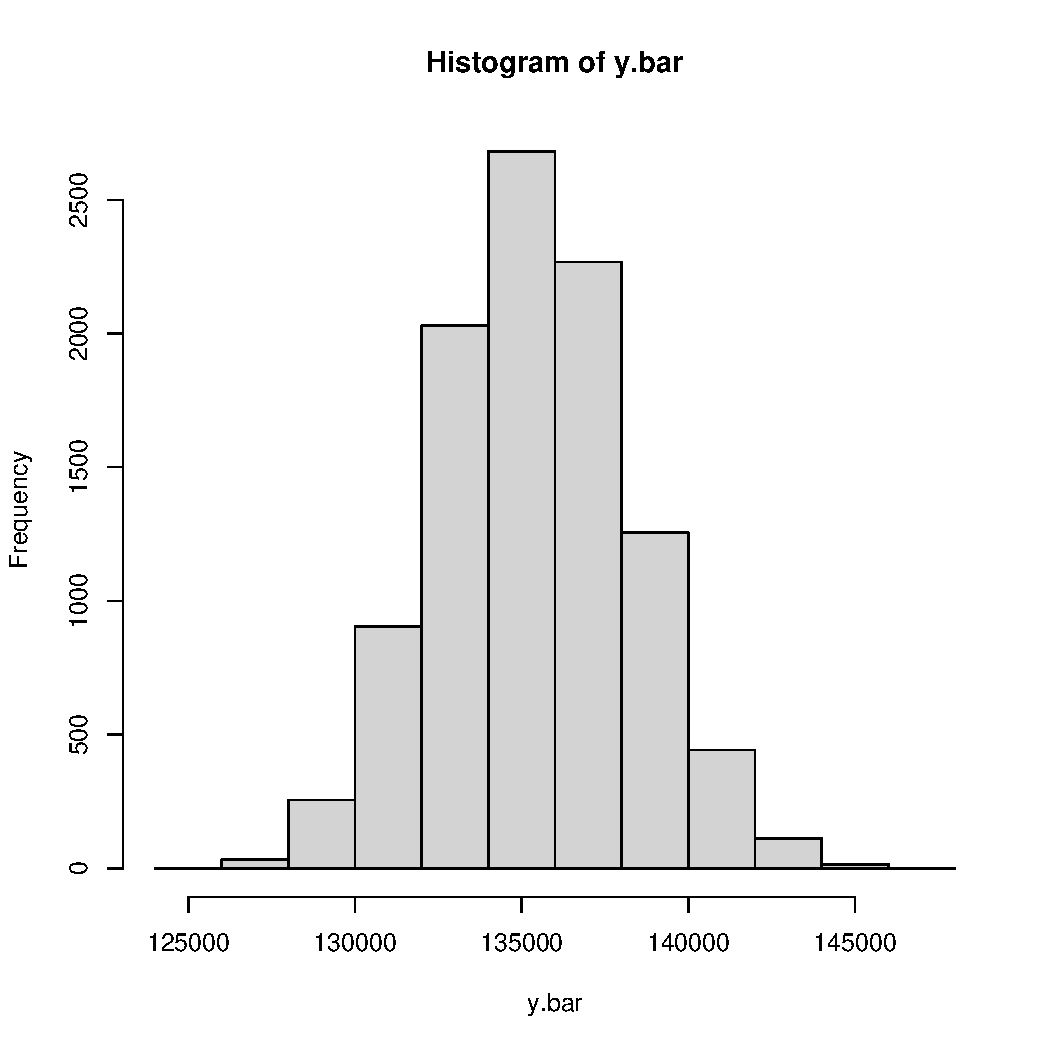
\includegraphics{figs/bootdist.pdf}}
\end{figure}

\begin{verbatim}
> quantile(y.bar,probs=c(.025,.975)) ## bootstrapped CI
    2.5%    97.5% 
129783.2 141169.0 
\end{verbatim} 

\end{frame}

\frame{
\frametitle{Bootstrapped Sampling Distribution vs Sampling Distribution}

\begin{enumerate}
\item CLT says the sampling distribution is approximately normal.
\item We see that the bootstrapped distribution is approximately normal.
\item Remaining question is whether the bootstrapped CI has approximately the same size as the middle 95\% of the sampling distribution.
\end{enumerate}

\bigskip

Let's table the remaining question for now while we look at another approach to CIs.

}


\frame{
\frametitle{Plug-in CI}

\begin{itemize}
\item Another way to get a 95\% CI is to use the fact that the middle 95\% of the distribution lies approximately between $\mu - 1.96 \cdot \frac{\sigma}{\sqrt{n}}$ and $\mu + 1.96 \cdot \frac{\sigma}{\sqrt{n}}$. 
\item If we denote the sample standard deviation with $s$, then we plug in sample values into the above statement: $\overline{y} - 1.96 \cdot \frac{s}{\sqrt{n}}$ and $\overline{y} + 1.96 \cdot \frac{s}{\sqrt{n}}$
\item 129,720 and 141,091 (note how close these are to the bootsrapped CI)
\end{itemize} \pause

\bigskip
\bigskip

Why does this work?
}

\frame{
The facts we've derived about the sampling distribution of the sample mean tell us that 
\begin{align*}
&P(\mu - 1.96 \cdot \frac{\sigma}{\sqrt{n}} \leq \overline Y \leq \mu + 1.96 \cdot \frac{\sigma}{\sqrt{n}}) \approx .95
\end{align*}
Some algebra (left as an exercise) shows that this implies 
\begin{align*}
&P(\overline Y - 1.96 \cdot \frac{\sigma}{\sqrt{n}} \leq \mu \leq \overline Y + 1.96 \cdot \frac{\sigma}{\sqrt{n}}) \approx .95
\end{align*}

\bigskip

Remaining question is whether $\frac{\sigma}{\sqrt{n}} \approx \frac{s}{\sqrt{n}}$ (note how similar this is to the remaining bootstrapped CI question).

}

\frame{
\frametitle{Partially Addressing Remaining Question}

\begin{itemize}
\item $\frac{\sigma}{\sqrt{n}}$ is called a standard error because it is the standard deviation for an estimator ($\overline Y$) of a parameter ($\mu$).
\item $\frac{s}{\sqrt{n}}$ is called an estimated standard error. We will bootstrap this estimated standard error to get a sense of its uncertainty (note the scale of this uncertainty). 
\end{itemize}

\begin{figure}[ht] \centering
        \scalebox{.3}{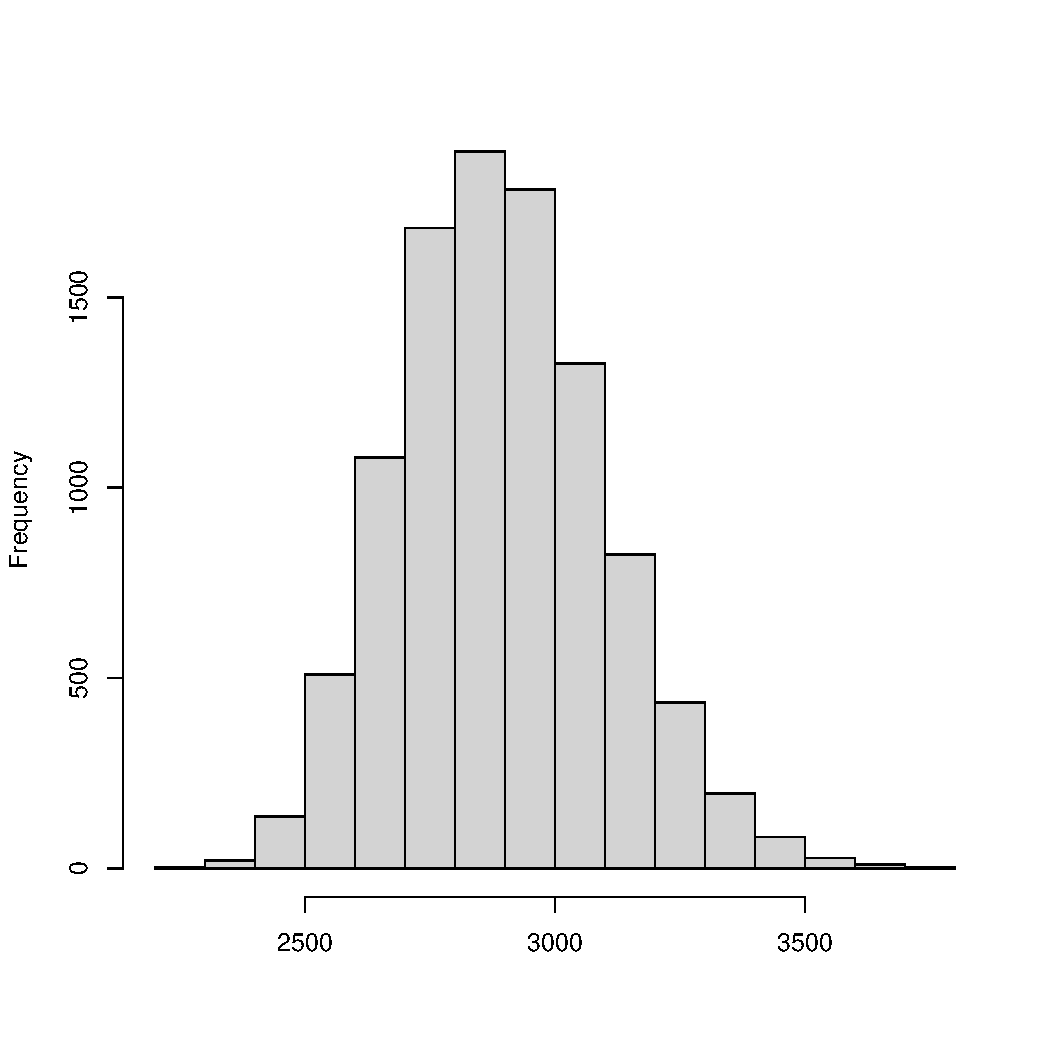
\includegraphics{figs/bootse.pdf}}
\end{figure}

}


\frame{
\frametitle{CI Wrap Up}

We got the following 95\% CIs for the population income mean:
\begin{itemize}
\item Boostrap: \$129,783 to \$141,169
\item Plug-in:  \$129,720 to \$141,091
\end{itemize} \pause
\bigskip
\bigskip


From the previous slide, we see the estimated standard error is very unlikely to be off by more than \$1,000, and therefore the bounds are very unlikely to be off by more than \$2,000. \pause

\bigskip
\bigskip

We are at least 95\% confident that the true population mean is roughly between \$128,000 and \$143,000, despite observing only a tiny fraction of the population.


}

\frame{
\frametitle{Two Questions}


\begin{enumerate}
\item Is \$135,406 close to the population mean $\mu$? \pause Yes! \pause
\item Can say something about how close? \pause Yes! Likely within \$7,500 or so. 
\end{enumerate} 

}

\frame{
\frametitle{Summary}

...
}


\end{document}

